\documentclass[11pt,letterpaper]{article}
\usepackage[utf8]{inputenc}
\usepackage{graphicx}
\usepackage{caption}
\usepackage{subcaption}
\author{Michael D. Brothers}
\title{Homework 7}
\begin{document}

\section{Problem 1.1.1}

\begin{figure}[!tbh]
    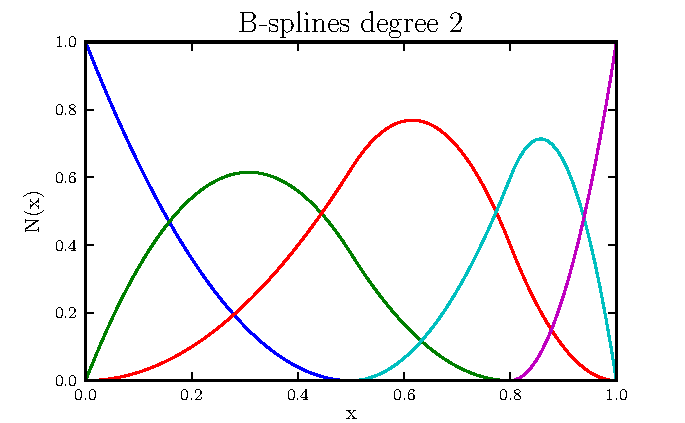
\includegraphics[width=\textwidth]{problem_1_1_1.pdf}
    \caption{\textbf{Zeros}: 
    The values of the basis functions are zero where they are defined to be zero, according to their Cox-DeBoor recursive definition in terms of box functions. 
    These box functions select over what intervals defined by the knot vector evaluate to nonzero for the given basis function. 
    The box functions can be determined easily by using a tree diagram created by inspecting the Cox-DeBoor formula for the desired basis function as was done in the handwritten component to this assignment.\\
    \textbf{Smoothness}:
    N1 is smooth from knot 1 to knot 2. N2 is smooth from knot 1 to knot 3. N3 is smooth from knot 1 to knot 4. N4 is smooth from knot 2 to knot 4. N5 is smooth from knot 3 to knot 4. 
    I say smooth since these functions are just polynomials over the intervals for which they are nonzero.}
    \label{fig1:label:a}

\end{figure}









\end{document}
